Lissajous curves are the result of two, or more, intersecting perpendicular sinusoidal curves. The most common occurrence of sinusoidal curves is in objects that exhibit simple harmonic motion, such as tuning forks or a pendulum as Jules-Antoine Lissajous did. Simple harmonic motion has been understood and researched for hundreds of years, and the equation can be found using Isaac Newton's second law. The equation for simple harmonic motion in a single direction is: \[x(t)=A \cos (\omega t-\varphi)\] Because a Lissajous curves consist of multiple instances of simple harmonic motion, they are mathematically represented as the following common paramaterization of the single direction formula: \[x=A \sin (a t+\delta), \quad y=B \sin (b t)\]
Changing the different components of the paramaterization affects the curve in different ways, from stretching to adding lobes. We will now go through how each variable affects the graph.

\subsection{Phase Shift: $\delta$}
The easiest way to understand these changes is visually. Below is a graph showing how phase increasing phase shift, moving clockwise, affects the curve described by the equation $x = \sin(2\pi t + \delta), \quad y = \sin(2\pi t)$. One interesting note on the phase shift, is that if you picture the curve as being in three dimensions, the phase shift then appears to rotate the curve either vertically or horizontally depending on the $\frac{a}{b}$ ratio, which will be discussed further below.
\begin{figure}[h]
    \centering
    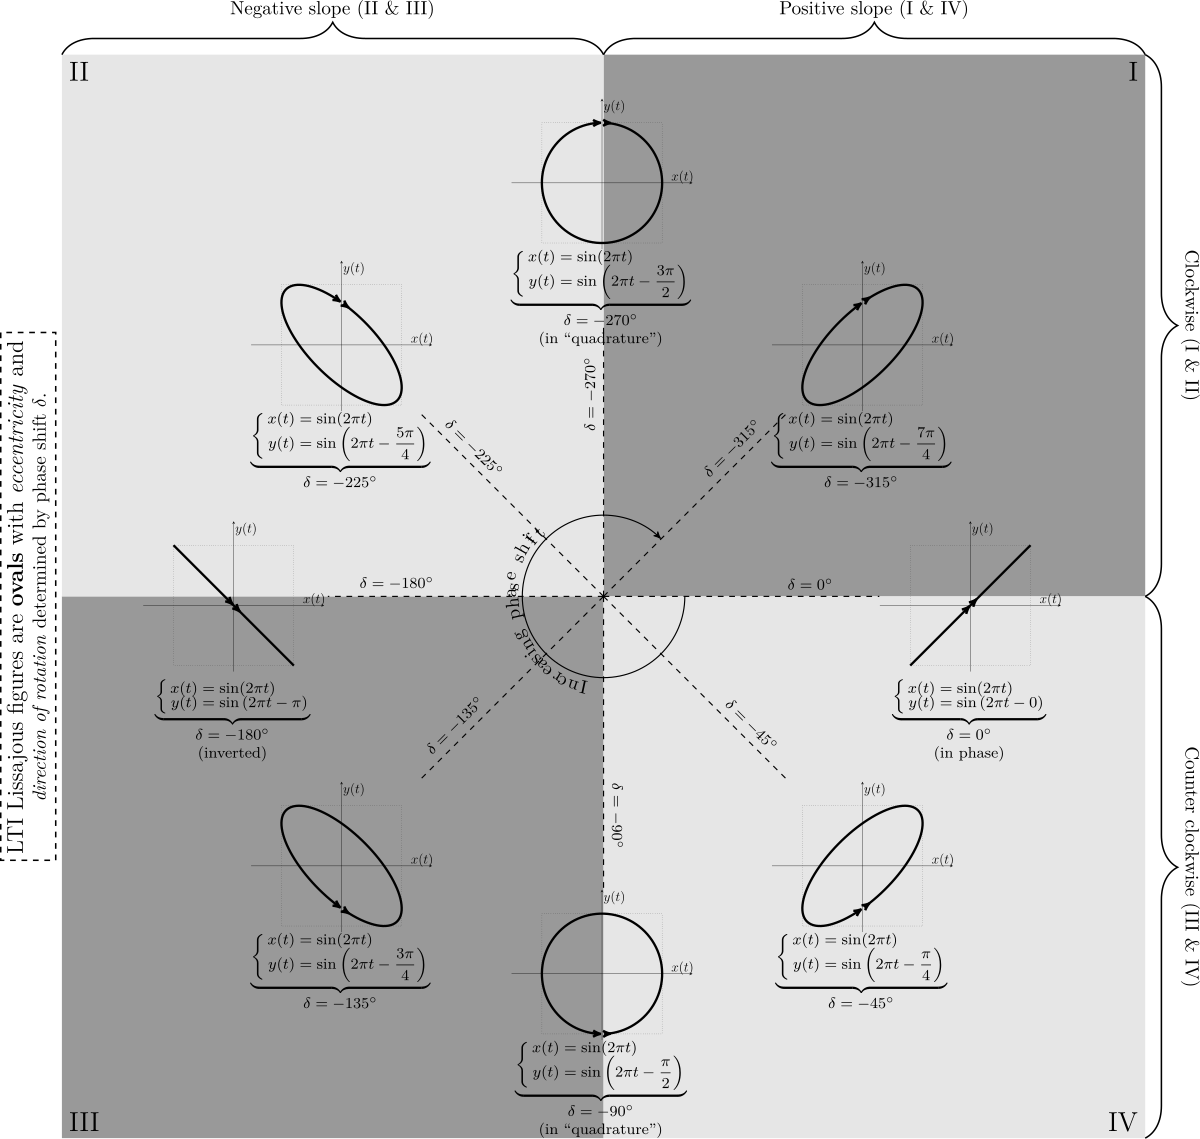
\includegraphics[scale=0.2]{Images/PhaseShift.png}
    \cite{PhaseShift}
    \caption{"Figure showing several Lissajous figures for different phase delays."}
    \label{fig:my_label}
\end{figure}
\newpage
\subsection{Amplitude: $A, B$}
In the single direction simple harmonic motion equation, these variables represent the magnitude of the motion. They act similarly here, but for their respective directions. The ratio $\frac{A}{B}$ represents the width to height ratio. \\ \\

\textbf{Changing A:}
\begin{center}
\begin{tikzpicture}[scale=1.4][h]
    \tkzInit[xmin=-3.5,xmax=3.5,xstep=1,ymin=-1.5,ymax=1.5,ystep=1]
    \tkzGrid[sub]
    \tkzAxeX[step=1]
    \tkzAxeY[step=1]
    \tkzFctPar[color = red, samples=200,domain=-pi:pi]{sin(t)}{sin(t+pi/2)}
    \tkzText[draw, above, color = red, fill = red!20](0.5,0){$A=1$}
    \tkzFctPar[color = blue, samples=200,domain=-pi:pi]{2*sin(t)}{sin(t+pi/2)}
    \tkzText[draw, above, color = blue, fill = blue!20](1.4,0){$A=2$}
    \tkzFctPar[color = green, samples=200,domain=-pi:pi]{3*sin(t)}{sin(t+pi/2)}
    \tkzText[draw, above, color = green, fill = green!20](2.3,0){$A=3$}
\end{tikzpicture}
\end{center}

\newpage
\textbf{Changing B:}
\begin{center}
\begin{tikzpicture}[scale=1.4][h]
    \tkzInit[xmin=-3,xmax=3,xstep=1,ymin=-3.5,ymax=3.5,ystep=1]
    \tkzGrid[sub]
    \tkzAxeX[step=1]
    \tkzAxeY[step=1]
    \tkzFctPar[color = red, samples=200,domain=-pi:pi]{sin(t)}{sin(t+pi/2)}
    \tkzText[draw, above, color = red, fill = red!20](0,0.5){$B=1$}
    \tkzFctPar[color = blue, samples=200,domain=-pi:pi]{sin(t)}{2*sin(t+pi/2)}
    \tkzText[draw, above, color = blue, fill = blue!20](0,1.4){$B=2$}
    \tkzFctPar[color = green, samples=200,domain=-pi:pi]{sin(t)}{3*sin(t+pi/2)}
    \tkzText[draw, above, color = green, fill = green!20](0,2.3){$B=3$}
\end{tikzpicture}
\end{center}

\subsection{Lobes: $a, b$}
These variables are perhaps the most interesting of the variables. The most obvious affect of changing these variables is the number of lobes. $a$ determines the number of vertical lobes, and $b$ determines the number of horizontal lobes. For the ratio $\frac{a}{b} = 1$, the curve produced is an ellipse, or, depending on the phase shift, a circle or line. Higher ratios result in more complex curves. As long as the ratio $\frac{a}{b}$ is rational, it will produce a closed figure, otherwise it will never loop back around. Below are some examples with different $\frac{a}{b}$ ratios.

\begin{figure}[h]
\begin{tikzpicture}[scale=0.8][h]
    \tkzInit[xmin=-2,xmax=2,xstep=1,ymin=-2,ymax=2,ystep=1]
    \tkzAxeX[step=1]
    \tkzAxeY[step=1,above]
    \tkzFctPar[color = red, samples=200,domain=0:2*pi]{sin(5*t+pi/4)}{sin(3*t)}
    \tkzText[draw, text width=2.6cm, above, left, color = red, fill = red!20](-2,2){$x = \sin(5t+\frac{\pi}{4}) \\ y = \sin(3t)$}
\end{tikzpicture}
\begin{tikzpicture}[scale=0.8][h]
    \tkzInit[xmin=-2,xmax=2,xstep=1,ymin=-2,ymax=2,ystep=1]
    \tkzAxeX[step=1]
    \tkzAxeY[step=1,above]
    \tkzFctPar[color = blue, samples=200,domain=0:8*pi]{sin(pi*t+pi/4)}{sin(2*t)}
    \tkzText[draw, text width=2.6cm, above, left, color = blue, fill = blue!20](-2,2){$x = \sin(\pi t+\frac{\pi}{4}) \\ y = \sin(2t)$}
\end{tikzpicture}
\begin{tikzpicture}[scale=0.8][h]
    \tkzInit[xmin=-2,xmax=2,xstep=1,ymin=-2,ymax=2,ystep=1]
    \tkzAxeX[step=1]
    \tkzAxeY[step=1,above]
    \tkzFctPar[color = green, samples=200,domain=0:2*pi]{sin(4*t)}{sin(3*t)}
    \tkzText[draw, text width=2.6cm, above, left, color = green, fill = green!20](-2,2){$x = \sin(4t) \\ y = \sin(3t)$}
\end{tikzpicture}
\hfill\begin{tikzpicture}[scale=0.8][h]
    \tkzInit[xmin=-2,xmax=2,xstep=1,ymin=-2,ymax=2,ystep=1]
    \tkzAxeX[step=1]
    \tkzAxeY[step=1,above]
    \tkzFctPar[color = purple, samples=200,domain=0:2*pi]{sin(t+pi/2)}{sin(3*t)}
    \tkzText[draw, text width=2.6cm, above, left, color = purple, fill = purple!20](-2,2){$x = \sin(t+\frac{\pi}{2}) \\ y = \sin(3t)$}
\end{tikzpicture}
\end{figure}

Many people draw parallels between these figures and three-dimensional knots, which is a valid connection. Many knots when projected into a plane are Lissajous curves, these are called Lissajous knots.
